\documentclass[../lab2.tex]{subfiles}

\begin{document}

    \begin{figure}[!htb]
        \begin{minipage}{0.48\textwidth}
            \centering
            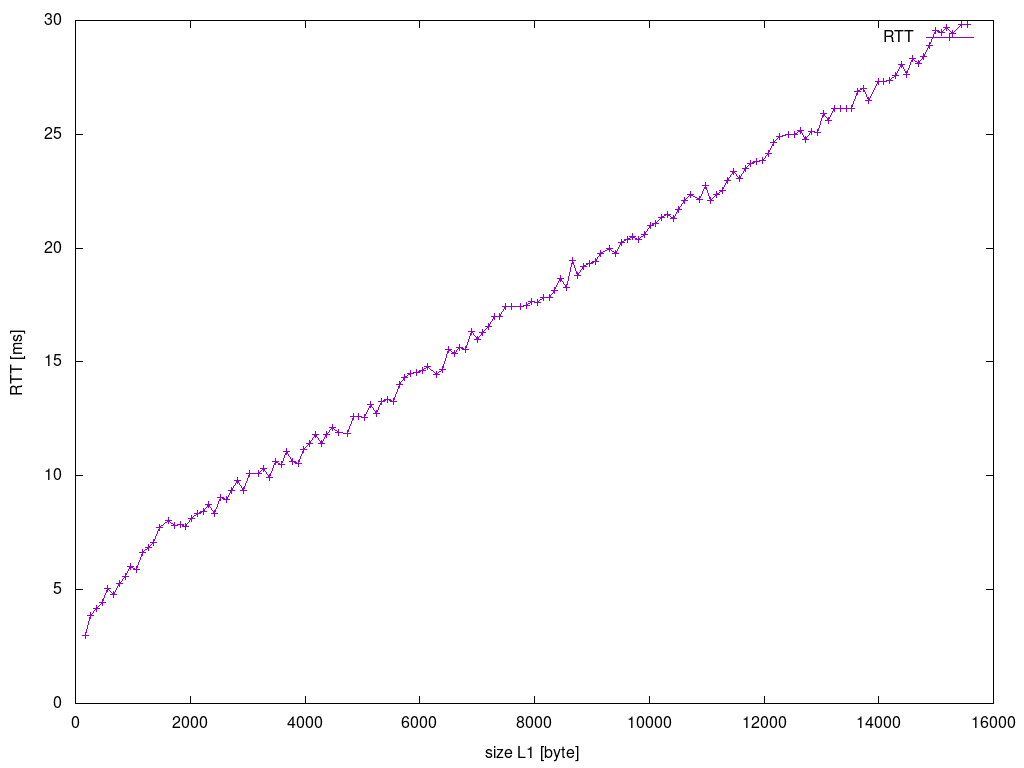
\includegraphics[width=1\linewidth]{RTTW.png}
            \vspace{-20pt}
            \caption{RTT}\label{RTTW}
        \end{minipage}\hfill
        \begin{minipage}{0.48\textwidth}
            \centering
            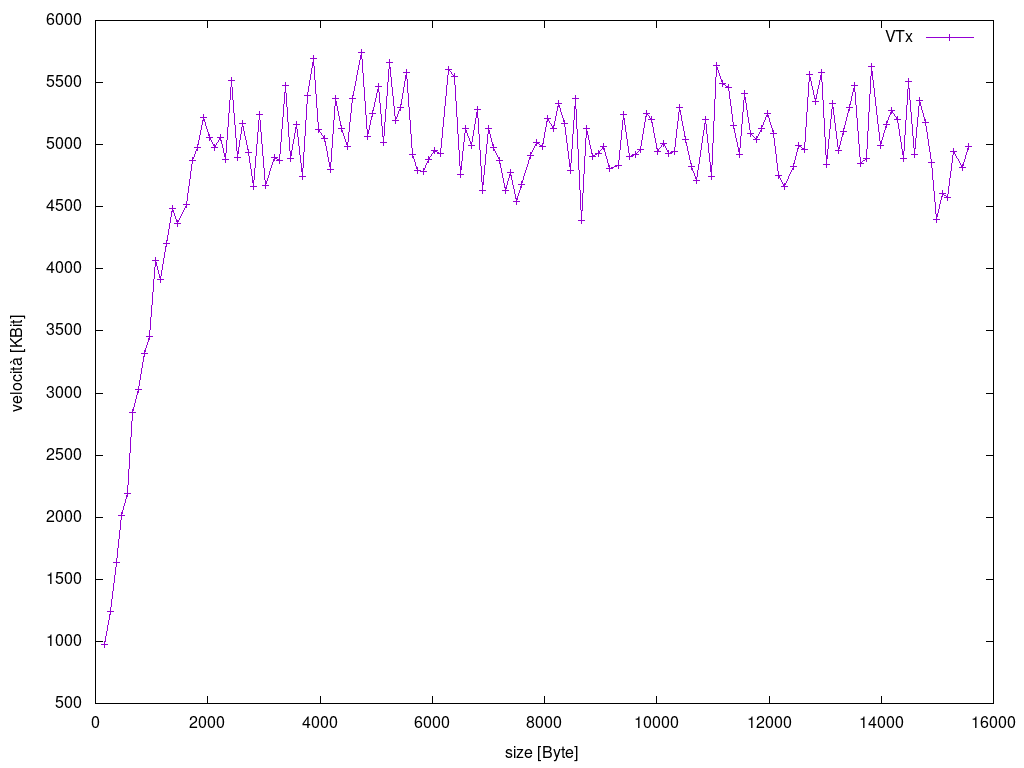
\includegraphics[width=1\linewidth]{VTxW.png}
            \vspace{-20pt}
            \caption{VTx}\label{VTxW}
        \end{minipage}
    \end{figure}

    Avendo impostato la velocita' di connessione tra Pc Live Linux e il router di 10Mb/s
    l'unica incognita rimane la velocita' della connessione wireless.
    Ipotizzando il caso in cui $V_{TX1} < V_{TX2}$, e' possibile ricavare:

    \begin{equation}
        \centering
        \begin{cases}
            RTT = \frac{2D}{V_{TX2}} +\frac{2D}{V_{TX1}} + T_\eta  \qquad \, \, \, D < 1500 \\
            \\
            RTT = \frac{2D}{V_{TX2}} +\frac{2MTU}{V_{TX1}} + T_\eta  \qquad D > 1500
        \end{cases}
    \end{equation}

    \begin{equation}
        \centering
        V_{TX1} = \frac{2D}{RTT - \frac{2MTU}{V_{TX2}}} 
    \end{equation}
    
    \vspace{10pt}

    Abbiamo riportato l'andamento della velocita' del WiFi approssimando l'header WiFi a
    40 Byte. \\
    Come si puo' notare analogamente ai punti precedenti all'aumentare della dimensione
    del pacchetto si arriva a una stima piu' accurata della velocita' poiche' si possono 
    trascurare con meno margine di errore i tempi di propagazione e elaborazione, 
    cioe' il fattore $T_\eta$.
    Dall'andamento del grafico si puo' notare una andamento un comportamento poco
    regolare probabilmente dovuto alla minore affidabilita' del mezzo trasmissivo 
    rispetto ad un cavo cablato.

\end{document}